\begin{flushright} {\tiny {\color{gray} \tt pair\_mtw.tex}} \end{flushright}
%~~~~~~~~~~~~~~~~~~~~~~~~~~~~~~~~~~~~~~~~~~~~~~~~~~~~~~~~~~~~~~~~~~~~~~~~~~~~~~~~~~~~~~~~~~~~~~~~~~

\begin{itemize}

%.........................................................
\item In \textcite{lomw12} we read:

\begin{displayquote}
{\color{darkgray}
The Mardal-Tai-Winther element was introduced in \textcite{matw02} (2002) as a finite element suitable
for the velocity space for both Darcy and Stokes flow in two dimensions. In the Darcy flow equations,
the velocity space only requires $H(\text{div})$-regularity. Moreover, discretizations based on $H^1$-conforming
finite elements are typically not stable. On the other hand, for the Stokes equations, the velocity 
space does stipulate $H^1$-regularity. The Mardal-Tai-Winther element is $H(\text{div})$-conforming, but
$H^1$-nonconforming. The element was extended to three dimensions in \textcite{tawi06} (2006).

\begin{center}
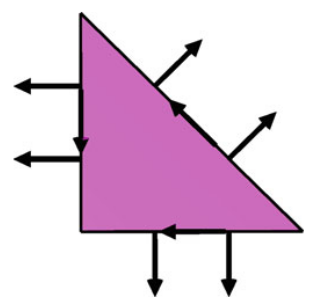
\includegraphics[width=4cm]{images/pair_mtw/mtw_lomw12}\\
{\captionfont 
Illustration of the Mardal-Tai-Winther element. The degrees of freedom are two moments
of the normal component on each facet and one moment of the tangential component on each facet.
In this figure, the moments of normal components are illustrated by point evaluation of normal
components.}
\end{center}

}
\end{displayquote}

%.........................................................
\item On the DefElement website\footnote{\url{https://defelement.org/elements/mardal-tai-winther.html}}
we find that it belongs to the 'Vector-valued elements' and  'H(div) conforming elements' categories.
It is also associated with the 'contravariant Piola' mapping.\todo{learn,explain}
It is available on triangles and tetrahedra.
On the site we find a degree 3 triangle and a degree 3 tetrahedron.


\begin{center}
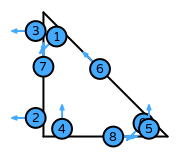
\includegraphics[width=3cm]{images/pair_mtw/element-Mardal-Tai-Winther-variant-equispaced-triangle-3-dofs}
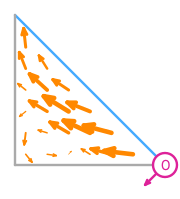
\includegraphics[width=3cm]{images/pair_mtw/element-Mardal-Tai-Winther-variant-equispaced-triangle-3-0}
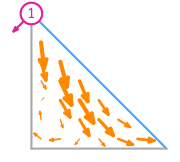
\includegraphics[width=3cm]{images/pair_mtw/element-Mardal-Tai-Winther-variant-equispaced-triangle-3-1}
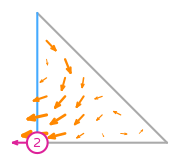
\includegraphics[width=3cm]{images/pair_mtw/element-Mardal-Tai-Winther-variant-equispaced-triangle-3-2}
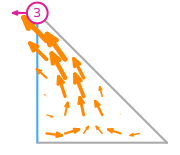
\includegraphics[width=3cm]{images/pair_mtw/element-Mardal-Tai-Winther-variant-equispaced-triangle-3-3}\\
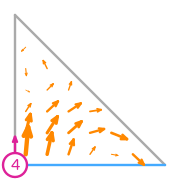
\includegraphics[width=3cm]{images/pair_mtw/element-Mardal-Tai-Winther-variant-equispaced-triangle-3-4}
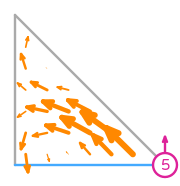
\includegraphics[width=3cm]{images/pair_mtw/element-Mardal-Tai-Winther-variant-equispaced-triangle-3-5}
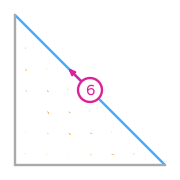
\includegraphics[width=3cm]{images/pair_mtw/element-Mardal-Tai-Winther-variant-equispaced-triangle-3-6}
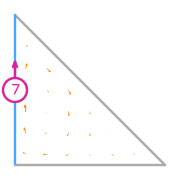
\includegraphics[width=3cm]{images/pair_mtw/element-Mardal-Tai-Winther-variant-equispaced-triangle-3-7}
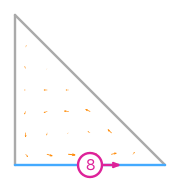
\includegraphics[width=3cm]{images/pair_mtw/element-Mardal-Tai-Winther-variant-equispaced-triangle-3-8}\\
{\captionfont Pink: degrees of freedom.}
\end{center}



${\cal V}$ is spanned by
\begin{small} 
\[
\left(\begin{array}{c}
1 \\ 0
\end{array}\right),
\left(\begin{array}{c}
 x \\ 0
\end{array}\right),
\left(\begin{array}{c}
y \\ 0
\end{array}\right),
\left(\begin{array}{c}
0 \\ 1
\end{array}\right),
\left(\begin{array}{c}
0 \\ x
\end{array}\right),
\left(\begin{array}{c}
0 \\ y
\end{array}\right),
\left(\begin{array}{c}
x(x+2y) \\ y (-2x-y)
\end{array}\right),
\left(\begin{array}{c}
x(-x^2+2x+3y^2) \\ y(3x^2-4x-y^2)
\end{array}\right),
\left(\begin{array}{c}
x(2xy+x+3y^2) \\ y(-2x-y)
\end{array}\right)
\]
\end{small}
with 
\begin{itemize}
\item DOF \#0 is associated with edge 0 of the reference element with $\vec{\bN}_0$ basis function.
\item DOF \#1 is associated with edge 0 of the reference element with $\vec{\bN}_1$ basis function.
\item DOF \#2 is associated with edge 1 of the reference element with $\vec{\bN}_2$ basis function.
\item DOF \#3 is associated with edge 1 of the reference element with $\vec{\bN}_3$ basis function.
\item DOF \#4 is associated with edge 2 of the reference element with $\vec{\bN}_4$ basis function.
\item DOF \#5 is associated with edge 2 of the reference element with $\vec{\bN}_5$ basis function.
\item DOF \#6 is associated with edge 0 of the reference element with $\vec{\bN}_6$ basis function.
\item DOF \#7 is associated with edge 1 of the reference element with $\vec{\bN}_7$ basis function.
\item DOF \#8 is associated with edge 2 of the reference element with $\vec{\bN}_8$ basis function.
\end{itemize}
and
\begin{eqnarray}
\vec{\bN}_0 &=&  \left(\begin{array}{c} 
x(30x^2+144xy-57x+126y^2-138y+23) \\ 
y(-90x^2-144xy+114x-42y^2+69y-25) 
\end{array}\right) \nn\\  
\vec{\bN}_1 &=&  \left(\begin{array}{c}  
x(-42x^2-144xy+69x-90y^2+114y-25)\\
y(126x^2+144xy-138x+30y^2-57y+23)
\end{array}\right) \nn\\  
\vec{\bN}_2 &=&  \left(\begin{array}{c}  
-24x^3-24x^2y+24x^2+36xy^2-24xy+4x+6y-4\\
2y(36x^2+12xy-24x-6y^2+6y-1)
\end{array}\right) \nn\\  
\vec{\bN}_3 &=&  \left(\begin{array}{c}  
48x^3+120x^2y-66x^2+36xy^2-60xy+16x-6y+2 \\
2y(-72x^2-60xy+66x-6y^2+15y-7)
\end{array}\right) \nn\\  
\vec{\bN}_4 &=&  \left(\begin{array}{c}  
\end{array}\right) \nn\\  
\vec{\bN}_5 &=&  \left(\begin{array}{c}  
\end{array}\right) \nn\\
\vec{\bN}_6 &=&  \left(\begin{array}{c}  
\end{array}\right) \nn\\
\vec{\bN}_7 &=&  \left(\begin{array}{c}  
\end{array}\right) \nn\\
\vec{\bN}_8 &=&  \left(\begin{array}{c} 
6x(4xy-x+6y^2-6y+1) \\ 
6y(-4xy+2x-2y^2+3y-1) 
\end{array}\right) \nn
\end{eqnarray}

 

































\end{itemize}

